\section{Basic control theory}
\todo[inline,color=other]{Varning! Utkast. Förvänta er fel!}


Control theory studies continuous systems and the control of these. A easy example of a control system, with human input, is when you take a shower. Your body sends signals to the brain when its to hot or cold and you adjust the temperature with your hand. In this case the input is the your hand adjusting the temperature and the output is the water temperature. This is a controls system with human input. In control theory we want to automate systems. Another example is the temperature in your house. A thermostat measures the outside and inside temperature and control the heat elements in you house. This is a control system with two inputs.

\begin{figure}[H]
    \centering
    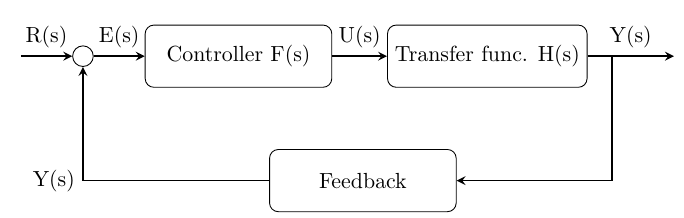
\includegraphics[]{feedback.PNG}
    \caption{Feedback-loop}
    \label{fig:feed}
\end{figure}


Control systems are created with the combination of measuring a magnitude and a controller. The magnitude measurements and controller create the system input u(t). The controller can also use the output and create a system with feedback. The quest for all control systems is to create a stable system without delay or overshoot. In the course ERE103 this is fulfilled by combining tree different parameters (P, I, D) to create controllers f(t).  P is just a constant and can decrease the delay of the system. P creates the most basic controller f(t) = Kp. The I parameter is the integrating part of the controller and is used to remove the stationary fault. The D parameter is used to avoid overshoot. The most common combination of these parameters in this course are PD, PI and PID.
\hrule
The systems are often modelled in block diagrams.
To decide if a system is stable different methods can be used. The characteristic equation, Ruth-Hurwitz or the Nyquist criteria. We will take a closer look at the Nyquist criteria. 

Bode diagram
Open loop/ Closed loop





